\documentclass{article}

\usepackage[romanian]{babel}
\usepackage[a4paper]{geometry}
\usepackage[hidelinks]{hyperref}

\usepackage{graphicx}

\title{{\huge ML}\\ Tema 2 --- Inteligență Artificială}
\author{Alexandru Sima (332CA)}

\begin{document}

\maketitle
\begin{abstract}
    Hello world!
\end{abstract}

\newpage
\tableofcontents

\newpage
\section{Poluarea aerului}
Primul set de date conține date despre diferiți parametri măsurați ai aerului,
în peste $20.000$ de orașe din întreaga lume. Prin antrenarea unui model de
învățare automată, se dorește clasificarea orașelor în funcție de gradul de 
riscuri pentru sănătate.

\subsection{Analiza datelor}
\subsubsection{Analiza valorică}
Setul de date conține 15 atribute, dintre care 7 numerice și 8 categorice 
(incluzând și atribul țintă "AQI\_Category").

\begin{figure}[ht]
    \centering
    \begin{tabular}{llllllll}
        & AQI\_Value & CO\_Value & Ozone\_Value & NO2\_Value & PM25\_Value & VOCs & SO2 \\
        înregistrări & 23463 & 23463 & 21117 & 23463 & 23463 & 23463 & 23463 \\
        val. medie & 72.01 & 1.36 & 35.23 & 43.08 & 68.51 & 185.05 & 4.44 \\
        dev. standard & 56.05 & 1.83&28.14 &196.07 &54.79&140.48&5.95 \\
        val. minimă & 6.00&0.00&0.00&0.00&0.00&12.41&-18.52\\
        cuartila 1 & 103.26&1.00&21.00&0.00&35.00&103.26&0.73\\
        mediana & 142.97&1.00&31.00&1.00&54.00&142.97&4.28\\
        cuartila 3 & 204.22&1.00&40.00&4.00&79.00&204.22&7.91\\
        val. maximă & 1280.98&133.00&222.00&1003.06&500.00&1280.98&234.69\\ 
    \end{tabular}
\end{figure}

TODO
\subsubsection{Echilibrul claselor}



\subsubsection{Corelația între atribute}
\subsubsection{Atribute numerice}
Aplicând testul Pearson pentru a determina corelația liniară dintre atributele 
numerice, se obține matricea din (\ref{fig:pol:corr}). Se poate presupune
astfel că atributele "AQI\_Value", "PM25\_Value" și "VOCs" sunt foarte puternic 
corelate între ele, având coeficientul de corelație $\geq 0.98$ și că atributul 
"NO2\_Value" nu este corelat cu niciun altul. Într-adevăr, primele 3 atribute 
sunt puternic corelate, acest fapt observându-se trasând graficele valorilor 
(\ref{fig:pol:corr_graphs}). Testul Pearson oferă însă doar informații despre
corelația liniară, astfel că, aplicând testul Spearman, se obține matricea din 
(\ref{fig:b}), care arată existența unor corelații între "NO2\_Value" și alți
parametri.

\begin{figure}[ht]
    \centering
    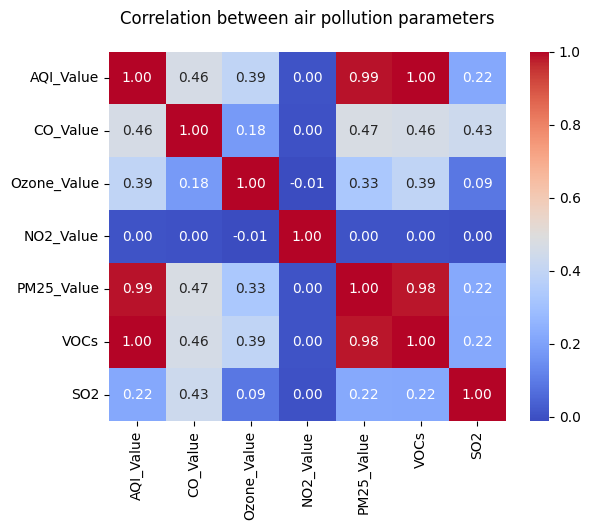
\includegraphics[scale=0.6]{images/air_pollution/correlation/matrix.png}
    \caption{Corelația dintre atributele dataset-ului}
    \label{fig:pol:corr}
\end{figure}

\begin{figure}[ht]
    \centering
    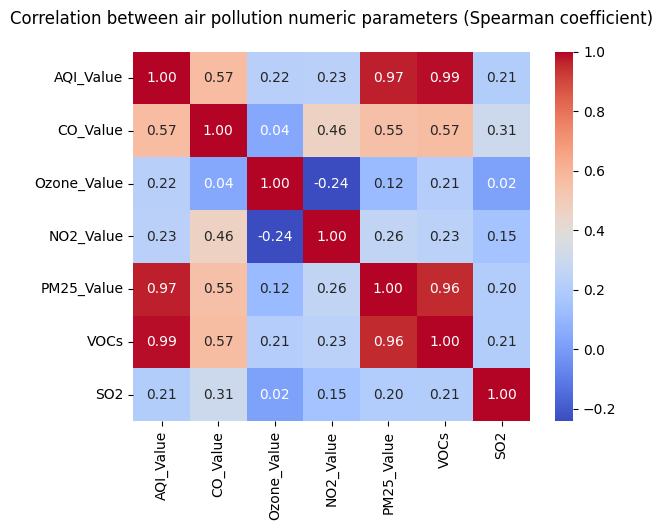
\includegraphics[scale=0.6]{images/air_pollution/correlation/matrix_spearman.png}
    \caption{Corelația dintre atributele dataset-ului, folosind coeficientul Spearman}
    \label{fig:b}
\end{figure}

\begin{figure}[ht]
    \centering
    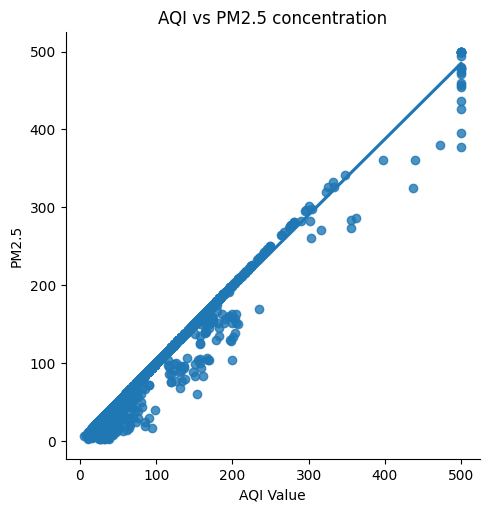
\includegraphics[scale=0.5]{images/air_pollution/correlation/aqi_pm25.png}
    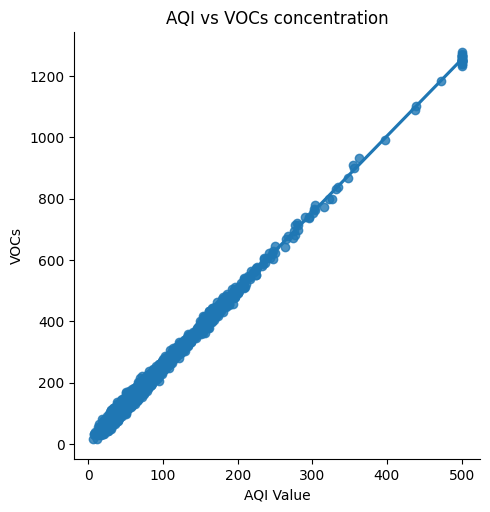
\includegraphics[scale=0.5]{images/air_pollution/correlation/aqi_vocs.png}
    \caption{Corelația liniară dintre AQI\_Value și PM25\_Value, respectiv VOCs}
    \label{fig:pol:corr_graphs}
\end{figure}

\subsection{Preprocesarea datelor}
\subsubsection{Imputarea valorilor lipsă}

\subsubsection{Eliminarea valorilor extreme}

\subsubsection{Eliminarea atributelor redundante}

Urmărind analiza corelației dintre atributele numerice efectuată la 
(\ref{fig:pol:corr}), se observă că atributele "AQI\_Value", "PM25\_Value" și 
"VOCs" sunt foarte puternic corelate, deci 2 dintre cele 3 pot fi eliminate. Am
ales să păstrez "AQI\_Value", neexistând diferențe semnificative între numărul 
de valori înregistrate ale fiecărui atribut sau distribuțiile acestora.

\subsubsection{Normalizarea datelor}

\subsection{Învățarea automată}

\end{document}